\chapter{Metode Penelitian}
Pada bab ini, akan dilakukan penjelasan mengenai alat dan bahan pendukung dari tugas akhir ini.
Alat dan bahan tersebut berupa perangkat keras, perangkat lunak, dan bahan data.
Selain itu, bab ini juga akan memaparkan mengenai alur dan urutan pengerjaan Tugas Akhir.
\section{Alat dan Bahan Tugas akhir}
Alat yang digunakan untuk mengembangkan Aplikasi ini terdiri dari Perangkat Keras dan Perangkat Lunak.
\subsection{Alat Tugas akhir}
\subsubsection{Perangkat Keras}
\begin{enumerate}
	\item \textit{laptop} dengan spesifikasi minimum anu, 
	pada tugas akhir ini digunakan \textit{Laptop Asus ROG Zephyrus G14} dengan spesifikasi sistem operasi Windows 11, \textit{processor} AMD Ryzen 5 4600HS with Radeon Graphics @ 3,00 GHz, memori 16GB DDR4, grafis NVIDIA GeForce GTX 1650Ti (4GB), SSD 512GB.
	\item \textit{Smartphone} dengan spesifikasi minimum anu, pada tugas akhir ini digunakan \textit{Smartphone Samsung Galaxy S20 Ultra} dengan spesifikasi OS Android 13 (Tiramisu), CPU Octa-core (2x2.73 GHz Mongoose M5, 2x2.50 GHz Cortex-A76, 4x2.0 GHz Cortex-A55), GPU Mali-G77 MP11, Internal 128 GB, 12GB RAM.
\end{enumerate}

\subsubsection{Perangkat Lunak}
\begin{enumerate}
	\item \textit{laptop} dengan spesifikasi minimum anu, 
	pada tugas akhir ini digunakan \textit{Laptop Asus ROG Zephyrus G14} dengan spesifikasi sistem operasi Windows 11, \textit{processor} AMD Ryzen 5 4600HS with Radeon Graphics @ 3,00 GHz, memori 16GB DDR4, grafis NVIDIA GeForce GTX 1650Ti (4GB), SSD 512GB.
	\item \textit{Smartphone} dengan spesifikasi minimum anu, pada tugas akhir ini digunakan \textit{Smartphone Samsung Galaxy S20 Ultra} dengan spesifikasi OS Android 13 (Tiramisu), CPU Octa-core (2x2.73 GHz Mongoose M5, 2x2.50 GHz Cortex-A76, 4x2.0 GHz Cortex-A55), GPU Mali-G77 MP11, Internal 128 GB, 12GB RAM.
\end{enumerate}
% \begin{enumerate}
% 	\item Microsoft Visual Studio Code 2022
% 	\item Figma
% \end{enumerate}
\newpage
\subsection{Bahan Tugas akhir}
Bahan yang digunakan untuk Tugas Akhir ini ialah sebagi berikut :
\begin{enumerate}
	\item Materi mata kuliah \textit{System Diagnosis Berbasis Pembantu Keputusan} (SBPK) dari Departemen Teknik Elektro dan Teknologi Informasi berupa file .pptx
	\item Data hasil wawancara pada Mahasiswa Teknik Biomedis sebagai informasi tambahan pembuatan \textit{User Persona}
	\item Data kuesiioner hasil pengujian \textit{System Usability Scale (SUS)} dan \textit{User Experience Questionnaire(UEQ)}
\end{enumerate}
% \begin{itemize}
% 	\item Dataset pihak lain yang diperoleh dengan izin atau dalam lisensi yang diizinkan untuk digunakan secara langsung 
% 	\item Dataset pihak pertama yang disusun sendiri melalui quisioner, observasi, atau interview 
% 	\item Dokumen panduan yang mengacu pada standar, hasil tugas akhir, atau artikel yang disitasi dan digunakan.
% \end{itemize}


\section{Metode yang Digunakan}
Metode yang digunakan dalam tugas akhir ini akan mengadopsi dari metode yang telah digunakan dalam penelitian-penelitian sebelumnya.
Dalam pengembangan desain, penelitian ini akan menggunakan metode pengembangan desain berbasis aktivitas atau \textit{Activity-centered Design}.
Metode ini digunakan karena proses pengembangan akan berfokus pada aktivitas utama dari pembelajaran \textit{Clinical Decision Support System}.
Selain itu juga, dalam proses pengembangan gamifikasi akan teratur berdasarkan setiap aktivitas yang sudah dirancang.
Metode pengembangan design ini akan bersinergi dengan pengembangan aplikasi yang akan digunakan yakni metode \textit{Feature-driven Development}.
\textit{Activity-Centered Design} dapat memberikan wawasan yang berharga dalam pemahaman pengguna, kebutuhan mereka, dan konteks penggunaan. 
Informasi ini dapat digunakan dalam identifikasi dan perencanaan fitur-fitur yang akan dikembangkan dalam pendekatan \textit{Feature-Driven Development}. 
Dengan memahami aktivitas pengguna secara mendalam, penulis dapat merancang dan mengembangkan fitur-fitur yang sesuai dengan kebutuhan pengguna.
Kedua proses desain dan pengembangan tersebut akan didasar oleh sebuah kerangka kerja gamifikasi. 
Kerangka kerja gamifikasi yang akan digunakan dalam tugas akhir ini ialah \textit{MDA Framework} atau \textit{Mechanics, Dynamics, and Aesthetics Framework}.
Pendekatan kerangka kerja ini digunakan karena bersifat komprehensif dan berfokus pada pengalaman pemain \cite{marisa2020gamifikasi}.

\section{Alur Tugas Akhir}
Penelitian ini akan dibagi menjadi tahap \textit{Design} dan implementasi desain gamifikasi, tahap \textit{Development} dan Tahap pengujian.
Metode yang digunakan pada tahap \textit{Design} aplikasi ini menggunakan metode design \textit{Activity-centered Design} 
dengan mengadopsi \textit{Framework Gamifikasi Mechanics, Dynamics, Aesthetics} untuk implementasi gamifikasi ke dalam desain tersebut.
Untuk tahap \textit{Development} perangkat lunaknya sendiri akan menggunakan metode \textit{Feature-Driven Development}.
Selanjutnya untuk akan dilakukan tahap pegujian, penulis akan mengujikan Fungsionalitas Aplikasi yang telah dikembangkan menggunakan Pengujian \textit{Black Box Testing}.
Kemudian dilanjutkan dengan Pengujian \textit{System Usability Scale} dan \textit{User Experience Questionnaire} untuk mengevaluasi pengalamaan pengguna mengenai Aplikasi yang telah dikembangkan.
Secara keseluruhan, Alur Tugas Akhir ini dapat dilihat secara lengkap pada gambar \ref{Fig:Alur Tugas Akhir}
\begin{figure}[H]
	\centering
	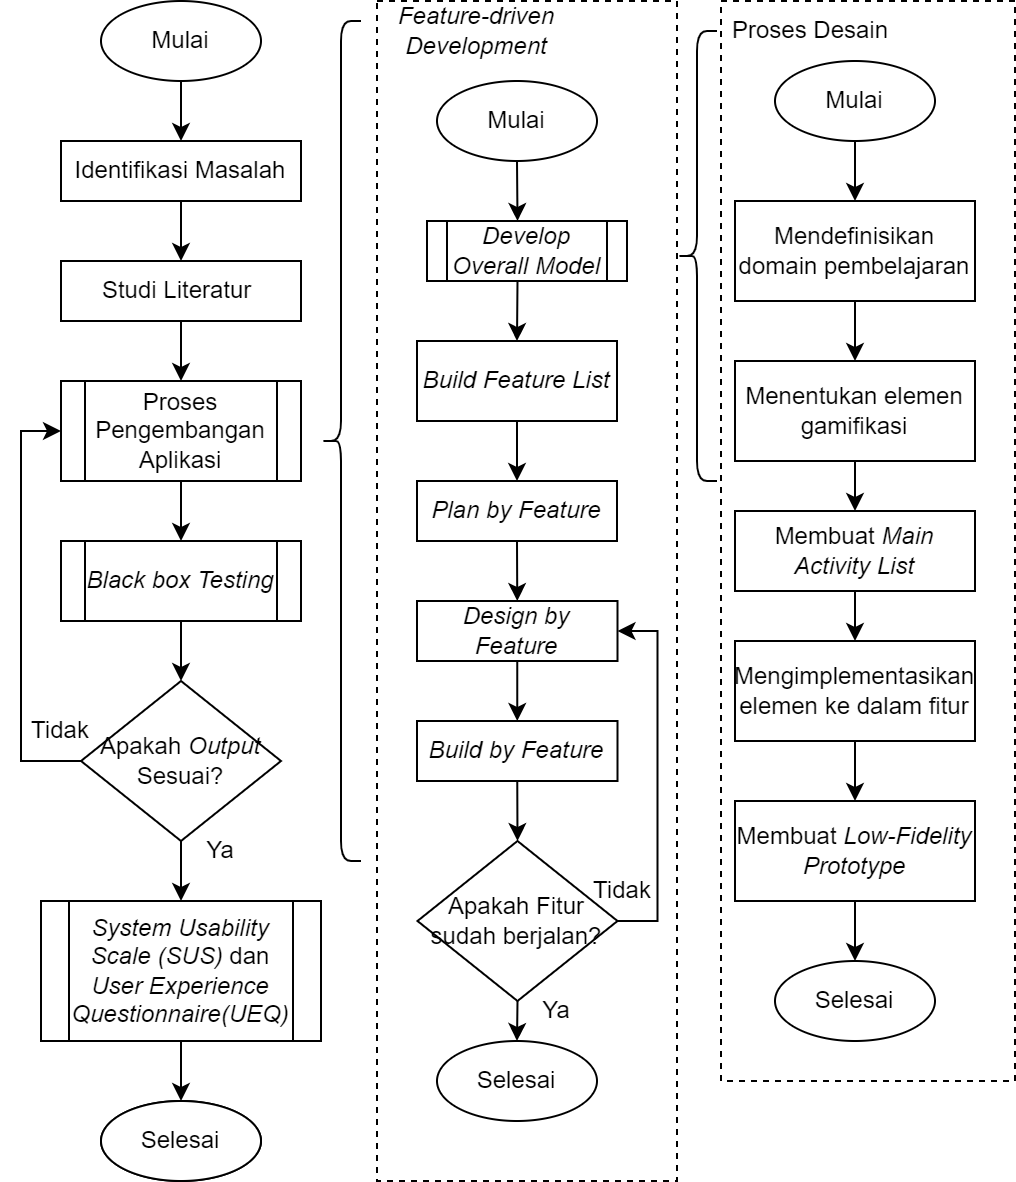
\includegraphics[width=\textwidth-1cm]{contents/chapter-3/images/Alur-tugas-akhir-2.png}
	\caption[Caption]{Alur Tugas Akhir}
	\label{Fig:Alur Tugas Akhir}
\end{figure}
% \section{Etika, Masalah, dan Keterbatasan Penelitian (Opsional)}
\subsection{Identifikasi Masalah}
Secara keseluruhan, penelitian ini akan membahas mengenai sebuah pembelajaran dalam sebuah ilmu yang spesifik, yaitu ilmu tentang \textit{Clinical Decision Support System}.
Hal yang pertama dilakukan dalam penelitian ini ialah mengidentifikasi masalah yang dihadapi sebagai motivasi awal penulis untuk melakuakn penelitian.
Identifikasi masalah dengan cara observasi mengenai masalah yang dihadapi dalam sebuah pembelajaran. 	

Observasi yang dilakukan ialah dengan mencari jurnal dan fakta terkait proses pembelajaran dan hubungannya dengan efektivitas pembelajaran.
Dalam penemuannya, salah satu masalah yang masih dihadapi dari sebuah proses pembelajaran ialah mengenai efektivitas pembelajaran yang dipengaruhi oleh motivasi dan kesiapan mahasiswa atau siswa \cite{hasan2021media}.
Pada sumber yang sama juga dijelaskan bahwa salah satu upaya untuk meningkatkan efektivitas sebuah pembelajaran ialah dengan menggunakan sebuah media pembelajaran yang tepat.
Penjelasn tersebut dijelaskan pada buku yang ditulis oleh Hasan(2021) yang berjudul "Media Pembelajaran"\cite{hasan2021media}.
Tentu saja demikian, bagaimana kita dapat mendapatkan ilmu jika kita sendiri tidak memiliki keinginan untuk mendapatkannya.
Salah satu strategi dalam menangani masalah tersebut ialah implementasi \textit{game desain} pada media pembelajaran tersebut \cite{EnjoyLearningLikeGaming}, tapi tidak sembarang \textit{game elemen} dapat dimasukan ke dalam sebuah media pembelajaran.
Pemilihan \textit{game element} yang tepat merupakan aspek penting dalam pengembangan media pembelajaran yang efektif\cite{kapp2012gamification}. Pernyataan tersebut mengarahkan penulis pada sebuah pertanyaan "Bagaimana memilih \textit{game element} yang tepat untuk sebuah media pembelajaran".

Ilmu yang dibahas pada penelitian ini akan lebih spesifik pada ilmu \textit{Clinical Decision Support System}. Ilmu ini merupakan salah satu ilmu yang sedang populer dan potensinya sangat besar dalam dunia medis \footnote[1]{Croskerry, Pat. "The theory and practice of clinical decision-making." Canadian Journal of Anesthesia 52.Suppl 1 (2005): R1-R8.}.
Ilmu ini tentu saja menarik untuk dipelajari mengingat potensinya yang besar dan masih bisa digali lagi, tapi masih belum ada media pembelajaran interaktif yang menyediakan pembelajaran mengenai ilmu ini.

Dari pernyataan-pernyataan tersebut, penulis dapat mengidentifikasi masalah yang dihadapi ialah media pembelajaran terkadang membosankan, dan hal tersebut akan berpengaruh ke dalam keefektivan pembelajran.
Selain itu, ilmu \textit{Clinical Decision Support System} belum menyediakan media pembelajran interaktif yang dapat menarik minat pengguna untuk mempelajarinya.
Dari masalah yang dihadapi, kemudian dapat dirumuskan kemungkinan solusi yang dapat menyelesaikan masalah tersebut. Salah satunya ialah dengan mengembangkan sebuah media pembelajaran yang secar spesifik membahas mengenai \textit{Clinical Decision Support System}.
Tidak samapai di sana, tentu saja media pembelajaran yang dikebangakan perlu memperhatikan faktor utama dari sebauh pembelajaran yaitu keefektivan pembelajaran.

\subsection{Studi Literatur}
Proses studi literatur pada penelitian ini dilakukan dengan tujuan untuk memperluas pemahaman mengenai isu yang serupa yang terjadi di lokasi lain, 
solusi pengembangan desain yang telah diimplementasikan oleh peneliti lain, serta implementasui gamifikasi yang melibatkan pemahaman tentang berbagai aspek, 
mulai dari jenis domain pembelajaran atau \textit{Type of Knowledge} hingga \textit{Framework} yang digunakan. 
Hal ini dilakukan melalui pembelajaran teori-teori, telaah buku, jurnal, dan sumber informasi lainnya yang relevan. 
Informasi yang diperoleh dari studi literatur tersebut akan menjadi dasar pertimbangan dalam mengembangkan fitur-fitur yang tepat untuk mengatasi masalah yang ada.
\subsection{\textit{Develop Overall Model}}
Setelah menelaaah literatur yanga ada, dilanjutkan dengan proses pengembangan. Proses pengembangan aplikasi ini dimulai dari mendesain model keseluruhan untuk sebuah aplikasi pembelajaran.
Sebelum melakukan proses desain, penulis akan menentukan domain ilmu yang akan dipelajari dalam sebuah media pembelajaran yang akan dikembangkan. Hal ini dimaksudkan untuk mempermudah untuk menetapkan elemen gamifikasi pada aplikasi tersebut.

Domain pembelajaran \textit{Clinical Decision Support System} dikategorikan sebagai \textit{Declarative Knowledge} karena tipe  mencakup pengetahuan tentang konsep-konsep dasar mengenai CDSS, seperti definisi CDSS, komponen-komponennya, prinsip-prinsip desain, dan metode evaluasi.
yang berhubungan dengan pengetahuan yang berkaitan dengan fakta, informasi, atau konsep yang dapat dinyatakan dengan jelas. Dalam CDSS, pengetahuan deklaratif mencakup pengetahuan medis dan informasi terkait yang digunakan untuk mendukung pengambilan keputusan klinis.
% Tujuan utama media pembelajaran ini ialah untuk memberikan informasi mengenai konsep dasar yang perlu diketahui dalam ilmu \textit{Clinical Decision Support System}.
% Penulis akan menggunakan domain pembelajaran atau \textit{Type of Knowledge} dari \textit{Clinical Decision Support System} dalam 
% Berdasarkan tabel hubungan domain learning dan gamifikasi, elemen gamifikasi untuk tipe \textit{Declarative Knowledge} adalah \textit{Stories/Narrative, Sorting, Matching,} dan \textit{Replayability}.
% Berdasarkan domain pembelajarannya, maka elemen gamifikasi yang akan diterapkan adalah sebagai berikut :
% \begin{itemize}
% 	\item \textit{Story} akan diimplementasikan dalam penjelasan materi konseptual \textit{Clinical Decision Support System} secara terurut
% 	\item \textit{Trivia} akan diimplementasikan dalam latihan dengan format kuis, atau jawaban pilihan ganda
% \end{itemize}
% kedua elemen tersebut meruapakan elemen inti gamifikasi yang akan diimplementasikan berdasarkan jenis pembelajarannya atau domain ilmunya yaitu \textit{Declarative Knowledge}.
\subsubsection{\textit{User persona}}
Sebelum melakukan proses desain, akan dibuat terlebih dahulu sebuah \textit{user persona} dari gambaran umum aplikasi yang akan dibuat.
\textit{User persona} adalah representasi fiktif dari pengguna ideal atau target yang dibuat berdasarkan analisis dan pemahaman tentang karakteristik, kebutuhan, dan tujuan pengguna yang sebenarnya. 
Pembuatan \textit{user persona} adalah untuk membantu dalam memahami target dan membantu dalam merancang pengalaman pengguna yang lebih relevan dan efektif.
Dalam penelitian ini, \textit{user persona} dibuat berdasarkan informasi yang didapatkan melalui wawancara salah satu target audiense yaitu selaku mahasiswa yang sudah pernah mempelajari \textit{Clinical Decision Support System}.

\begin{figure}[H]
	\centering
	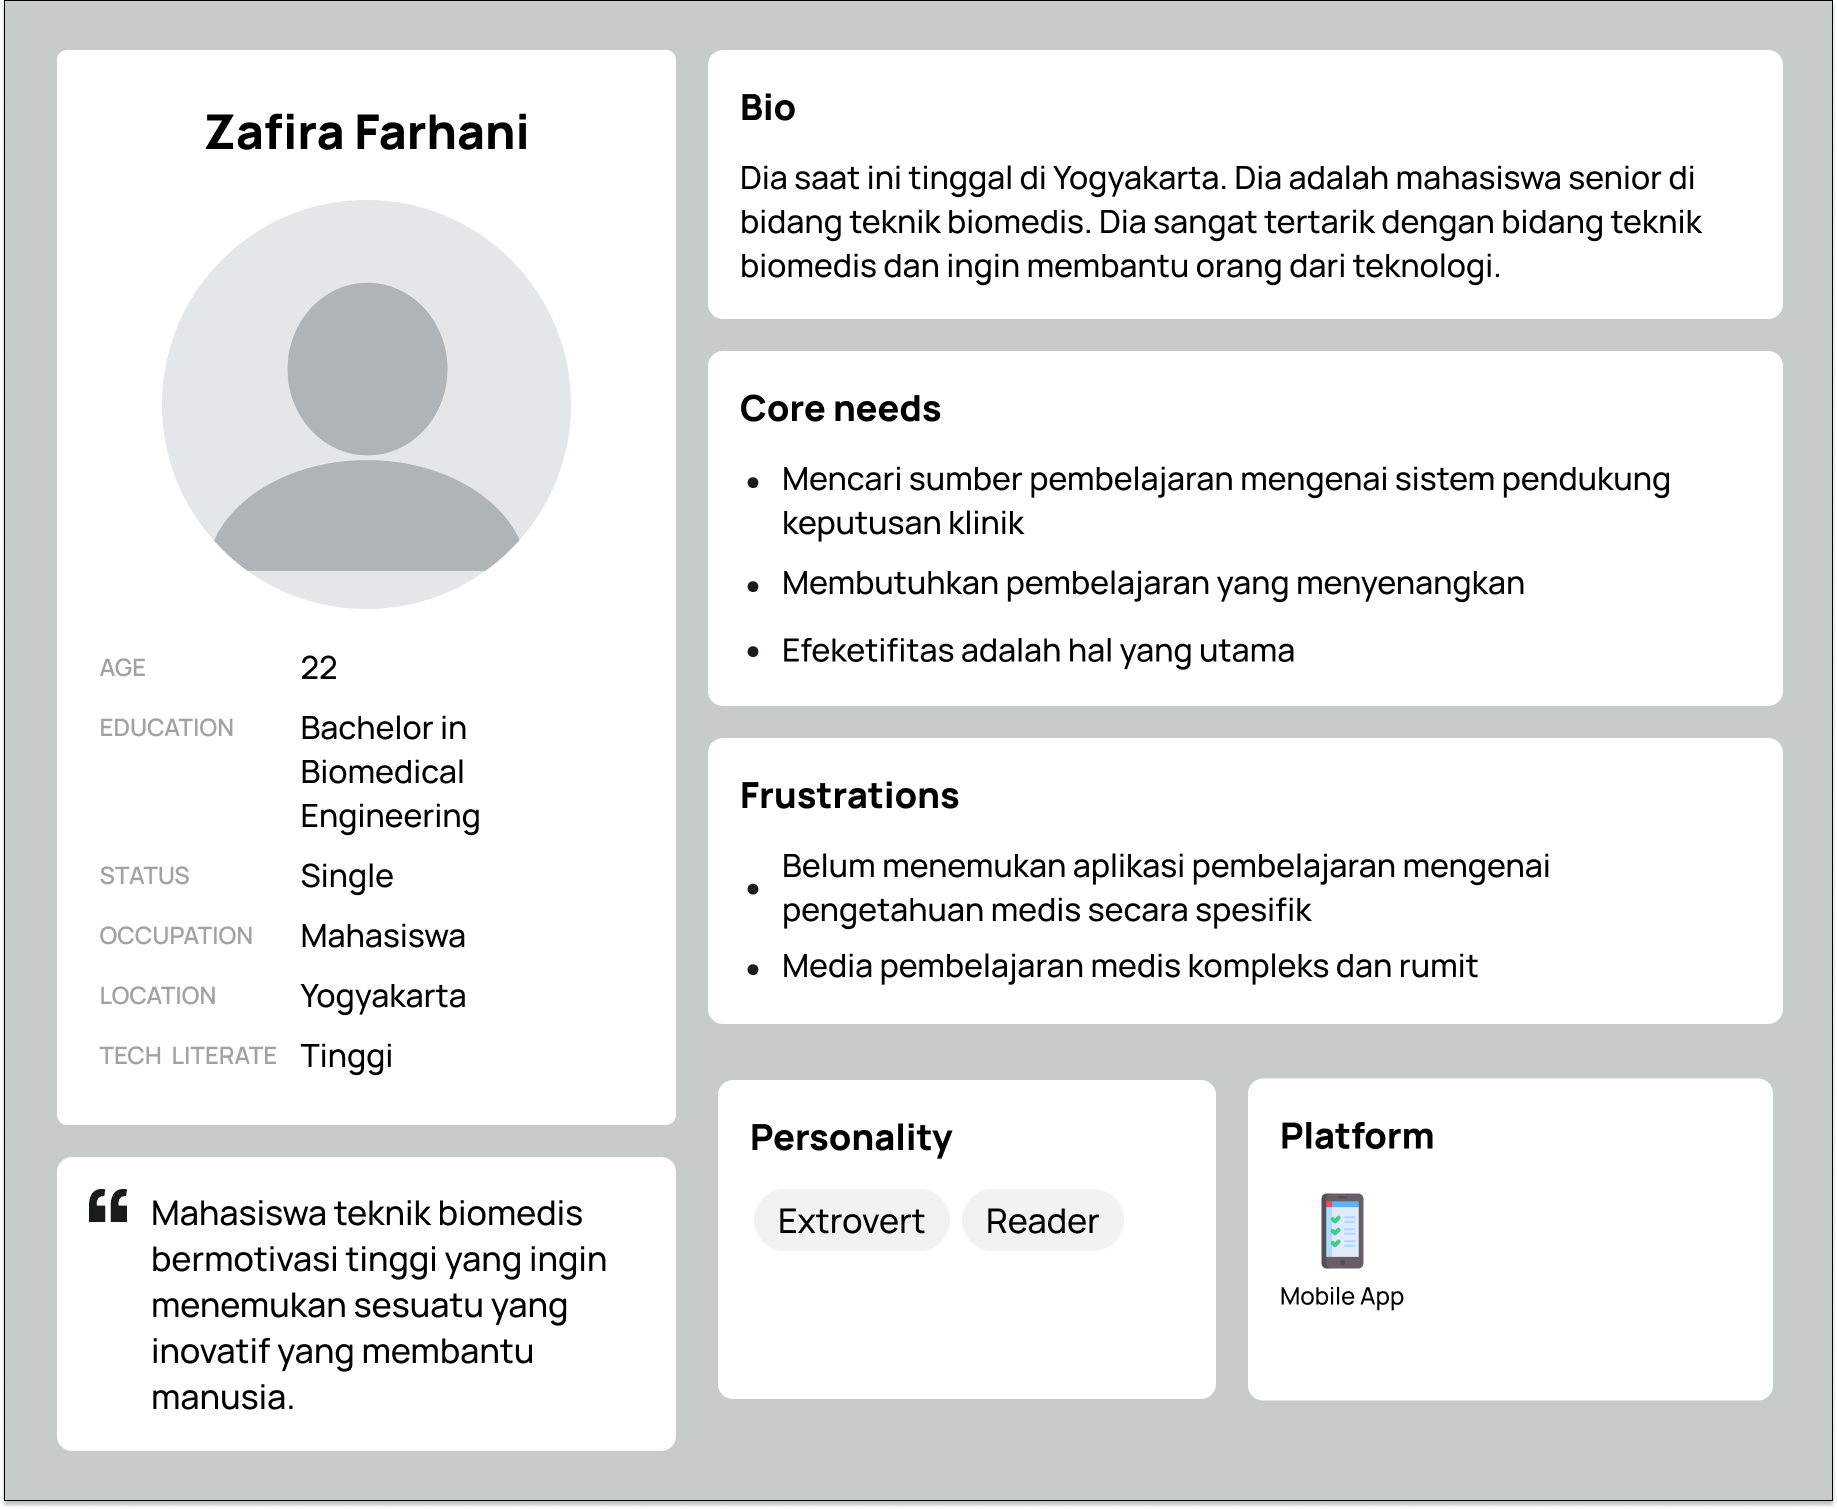
\includegraphics[width=\textwidth]{contents/chapter-3/images/up-dummy.png}
	\caption[Caption]{User Persona}
	\label{Fig:UserPersona}
\end{figure}
\subsubsection{\textit{Activity-centered Design}}
% Selanjutnya ialah proses pengembangan desain dengan menggunakan metode bernama \textit{Activity-centered Design}.
% Desain dikembangkan berdasarkan \textit{Main Activity} atau aktivitas utama yang akan dilakukan user dalam melakukan pembelajaran.
\begin{table}[H]
	\centering
	\caption{Struktur aktivitas utama}
	\begin{tabular}{|m{1cm}|m{0.9\textwidth}|}
		\hline
		\textbf{ID} & \multicolumn{1}{c|}{\centering \textbf{Aktivitas Utama}}\\
		\hline
		A-01 & \textit{Google Sign-in} \\
		\hline
		A-02 & Melihat \textit{dashboard} halaman utama\\
		\hline
		A-03 & Mempelajari materi\\
		\hline
		A-04 & Mengerjakan kuis singkat mengnai materi \\
		\hline
		A-05 & Melihat urutan \textit{Leaderboard} dari kuis terkait\\
		\hline
		A-06 & Melihat penghargaan atau \textit{Achievement} berdasarkan kuis terkait \\
		\hline
		A-07 & \textit{Log-Out}\\
		\hline
	\end{tabular}
	\label{Tab: Tabel Main Activity}
\end{table}
Tabel \ref*{Tab: Tabel Main Activity} merupakan daftar aktivitas utama untuk aplikasi yang akan dikembangkan.
Secara keseluruhan aplikasi pembelajaran yang akan dikembangakan memiliki tujuan untuk mempelajari \textit{Clinical Decision Support System} dimana aktivitasanya utamanya diantaranya mempelajari materi, dan melakukan kuis untuk melatih pemahaman.
Dari daftar aktivitas tersebut, kemudian dirancang sebuah \textit{Use Case Diagram} sebagai gambaran umumnya (gambar \ref*{Fig:Use Case Diagram}). 
\begin{figure}[H]
	\centering
	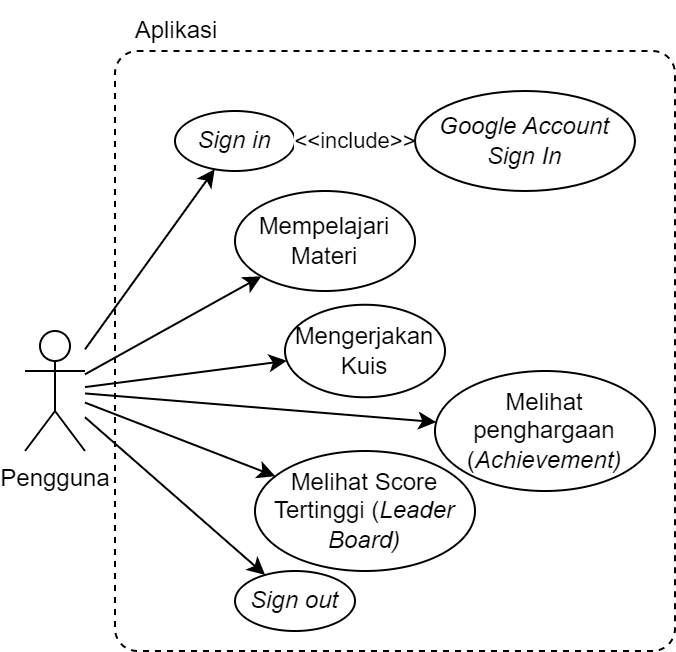
\includegraphics[width=0.7\textwidth]{contents/chapter-3/images/Use-Case-Diagram.png}
	\caption[Caption]{\textit{Use Case Diagram}}
	\label{Fig:Use Case Diagram}
\end{figure}

\subsubsection{\textit{Gamification Design}}
Proses pengembangan gamifikasi dalam aplikasi ini akan mengikuti kategori domain pembelajaran atau \textit{Type of Knowledge}. Seperti yang sudah dijelasakan sebelumnya, Domain pembelajaran ilmu \textit{Clinical Decision Support System} dapat dikategorikan sebagai \textit{Declarative Knowledge}.
Tipe kategori \textit{Declarative Knowledge} memiliki definisi sebagai declarative knowledge dapat didefinisikan sebagai jenis pengetahuan yang mencakup fakta-fakta, konsep-konsep, prinsip-prinsip, dan aturan-aturan yang dapat dinyatakan secara eksplisit.
Dalam buku yang ditulis oleh Kapp(2012), setiap domain pembelajaran memiliki elemen gamifikasinya masing-masing. Dalam bukunya menjelaskan domain \textit{Declarative Knowledge} memiliki elemen gamifikasi \textit{Story/Narrative}, \textit{Sorting}, \textit{Matching}, dan \textit{Replayability}.
Lebih lengkapnya pada tabel \ref*{Tab:Declarative-knowledge}
\begin{table}[H]
	\centering
	\caption{Domain \textit{Declarative Knowledge}}
	\begin{tabular}{|p{2.7cm}|p{3cm}|p{2.7cm}|p{2.7cm}|p{2cm}|}
		\hline
		\centering\textbf{Domain Pembelajaran} &\centering\textbf{Definisi}  &\centering\textbf{Strategi Instruksi}  &\centering\textbf{Elemen Gamifikasi} &\multicolumn{1}{m{2cm}|}{\centering \textbf{Contoh}}\\
		\hline
		\textit{Declarative Knowledge} 
		&Asosiasi antara dua atau lebih objek. Ini biasanya berupa fakta, istilah khusus, dan singkatan. Kontennya harus dihafal.
		&Elaborasi, Pengorganisasian, Asosiasi, Pengulangan
		&\textit{Story/Narrative}, \textit{Sorting}, \textit{Matching}, dan \textit{Replayability}
		&\textit{Trivia, Hang-man, Drag and Drop} \\
		\hline
	\end{tabular}
	\label{Tab:Declarative-knowledge}
\end{table}
Dari hubungan tersebut, elemen gamifikasi yang akan digunakan ialah \textit{Story/Narrative} dan akan dikemas dalam bentuk materi yang dapat diakses secara berurutan mengenai \textit{Clinical Decision Support System}. Selain itu, elemen tersebut dapat dikemas dalam sebuah kuis singkat untuk menguji pemahaman.
Kuis yang dapat dilakukan dapat dikerjakan secara berulang ulang sehingga memenuhi elemen gamifikasi \textit{Replayability}. Kedua elemen ini, ialah elemen utama yang kemudian akan dikembangkan lagi dalam kerangka kerja gamifikasi.
Proses pengembangan gamifikasi akan menggunkan pendekatan kerangka kerja \textit{MDA} yang terdiri dari \textit{Mechanics, Dynamics, and Aesthetics}. 
Penggunaan metode dan rancangan ini disesuaikan dengan kebutuhan dan tujuan adanya gamifikasi dalam aplikasi yang dikembangkan.
Acuan pengembangan desain ini akan mengikuti dengan Aktivitas Utama yang sudah dirumuskan sebelumnya pada tabel \ref*{Tab: Tabel Main Activity}.
Pengembangan ini dimulai dari pengembangan \textit{Game Mechanics}.

\textit{Game Mechanics} berfokus pada aturan pada peraturan pada permainan. Mekanika permainan yang tersusun pada aplikasi ini ialah :
\begin{description}
	\item[\textit{Modes}]
	pada aplikasi, akan tedapat 2 mode, yaitu pembelajaran materi dan Kuis.
	Pembelajaran materi melibatkan materi-materi dasar mengenai \textit{Clinical Decision Support System}. Pengguna dapat membaca materi secara berurutan dimulau dari konsep umum \textit{DSS},\textit{CDSS}, \textit{Medical Diagnostic Test}, dan \textit{Electronic Health Record}.
	Selain itu ada mode kuis yang
	merupakan elemen mekanik yang melibatkan pertanyaan dan jawaban. Pengguna dapat menguji pengetahuan mereka dan mendapatkan poin atau penghargaan berdasarkan hasil kuis yang mereka jawab dengan benar.
	\item[\textit{Points}] merupakan elemen mekanik yang digunakan untuk memberikan insentif kepada pengguna dalam menyelesaikan tugas atau mencapai tujuan tertentu. Poin dapat diberikan berdasarkan aktivitas atau pencapaian tertentu dalam aplikasi Anda.
	\item[\textit{Achievement}] merupakan elemen mekanik yang memberikan penghargaan kepada pengguna ketika mereka mencapai tujuan atau melakukan pencapaian tertentu dalam aplikasi. Pencapaian ini dapat berupa sertifikat, badge, atau level yang diberikan kepada pengguna sebagai bentuk pengakuan atas prestasi mereka.
\end{description}
Selanjutnya stelah mendesain mekanika game, dilanjutkan dengan mendesain dinamika permainan. \textit{Dynamics} atau Dinamika merujuk pada perilaku sistem permainan yang timbul dari interaksi antara pemain dengan mekanika permainan. Ini mencakup respons terhadap tindakan pemain, aliran permainan, pola interaksi, dan perubahan yang terjadi seiring permainan berlangsung. Dinamika permainan yang tersusun pada aplikasi ini ialah : 
\begin{description}
	\item[{Materi yang diakses berurutan}] merupakan elemen dinamis yang melibatkan pengguna dalam mengeksplorasi dan memperoleh pengetahuan secara berurutan. Pengguna dapat menavigasi melalui materi yang disusun dengan urutan tertentu untuk memahami konten aplikasi secara sistematis.
	\item[\textit{Leaderboard}] Merupakan elemen dinamis yang memungkinkan pengguna untuk melihat peringkat mereka dan peringkat pengguna lain dalam aplikasi. Ini menciptakan dinamika persaingan di antara pengguna, mendorong mereka untuk mencapai skor tinggi dan berada di peringkat teratas.
\end{description}
Akhir dari kerangka kerja ini kemudian dilanjutkan dengan mendesain estetika permainan. \textit{Aesthetics} atau estetika merujuk pada perasaan, emosi, dan kepuasan yang dirasakan oleh pemain saat bermain. Estetika memberikan dimensi pengalaman permainan yang melibatkan elemen seperti kegembiraan, kepuasan, kekaguman, dan tantangan. Estetika permainan yang tersusun pada aplikasi ini ialah : 
\begin{description}
	\item [\textit{Unlocking Part}] berdasarkan urutan, diharapkan pengguna mendapatkan perasaan untuk membuka materi baru.
	\item [\textit{On Boarding}] sebagai panduan kepada pengguna baru untuk membantu pengguna mengikuti dinamika permainan yang dibuat.
	\item [\textit{Desain Visual}] sebagai elemen antarmuka yang melibatkan tampilan dan estetika aplikasi Anda. Desain visual yang menarik dan konsisten dapat meningkatkan pengalaman pengguna dan membuat aplikasi lebih menarik.
\end{description}
Setelah mendesain keseluruhan gamifikasi, proses selanjutnya ialah menuliskan daftar fitur yang akan diimplementasikan dalam aplikasi yang dikembangkan.
Penulisan daftar fitur ini tentunya merupakan fitur yang sudah dimodifikasi dengan elemen gamifikasi 
atau bisa disebut dengan pengembangan aktivitas utama yang sudah melalui proses gamifikasi.
\newpage
\subsection{\textit{Build Feature List}}
Proses \textit{Build Feature List} akan menuliskan daftar fitur yang dikembangkan dari desain gamifikasi yang sudah dibuat.
Daftar-daftar yang akan dijelaskan ini adalah perkembangan aktivitas yang lebih detail dari aktivitas utama pada tabel \ref*{Tab: Tabel Main Activity}.
Dengan demikian, fitur aktivitas utama akan menjadi kelompok fitur set yang memiliki bagian-bagian fitur lainnya.
\begin{table}[H]
	\centering
	\caption{Daftar Fitur}
	\begin{tabular}{|m{3cm}|p{0.68\textwidth}|m{1.5cm}|}
		\hline
		\centering\textbf{Aktivitas Utama} & \centering\textbf{Fitur} & \multicolumn{1}{m{1.5cm}|}{\centering \textbf{ID}} \\
		\hline
		\multirow{4}{2.5cm}{\textit{Sign-in}} &Menampilkan halaman Sign-in & F-01 \\
		\cline{2-3}
		 &Mencatat \textit{user} baru ketika melakukan \textit{Sign-in} pertama & F-02 \\
		\cline{2-3}
		 &Aplikasi dapat memberikan akses pengguna ketika pengguna sudah terdaftar& F-03 \\
		\hline
		\multirow{5}{2.5cm}{Melihat \textit{dashboard} halaman utama} &Menampilkan halaman \textit{On Boarding} jika \textit{useer} belum terdaftar & F-04 \\
		\cline{2-3}
		&Menampilkan halaman utama aplikasi& F-05 \\
		\cline{2-3}
		&Menampilkan \textit{side drawer}& F-06 \\
		\cline{2-3}
		&\textit{Dialog box Sign Up} jika memilih fitur, tapi \textit{user} belum terdaftar& F-07 \\
		\cline{2-3}
		&Memilih fitur kuis dan fitur materi& F-08 \\
		\hline
		\multirow{6}{2.5cm}{Mempelajari materi} &Menampilkan halaman daftar materi yang tersedia& F-09 \\
		\cline{2-3}
		&Menampilkan materi yang dipilih & F-10 \\
		\cline{2-3}
		&Keluar dari materi yang dipilih& F-11 \\
		\cline{2-3}
		&Fitur kunci materi jika materi sebelumnya belum dibaca& F-12 \\
		\cline{2-3}
		&Keluar dari halaman daftar materi dan kembali ke halaman utama& F-13 \\
		\hline
		\multirow{7}{2.5cm}{Mengerjakan kuis singkat mengnai materi} &Menampilkan halaman daftar kuis& F-14 \\
		\cline{2-3}
		&Menampilkan halaman kuis yang dipilih& F-15 \\
		\cline{2-3}
		&Memilih salah satu jawaban kuis berbasis pilihan ganda& F-16 \\
		\cline{2-3}
		&Menampilkkan halaman kuis nomor selanjutnya& F-17 \\
		\cline{2-3}
		&Menampilkan halaman kuis nomor sebelumnya& F-18 \\
		\cline{2-3}
		&Menampilkan ringkasan kuis& F-19 \\
		\cline{2-3}
		&Menyelesaikan kuis& F-20 \\
		\hline
	\end{tabular}
\end{table}

\newpage
\begin{table}[H]
	\begin{tabular}{|m{3cm}|p{0.68\textwidth}|p{1.5cm}|}
		\hline
		\centering\textbf{Aktivitas Utama} & \centering\textbf{Fitur} & \multicolumn{1}{m{1.5cm}|}{\centering \textbf{ID}} \\
		\hline
		\multirow{8}{2.5cm}{Mengerjakan kuis singkat mengnai materi} &Menampilkan halaman daftar kuis& F-14 \\
		\cline{2-3}
		&Mendapatkan score kuis& F-21 \\
		\cline{2-3}
		&Mencatat score kuis& F-21 \\
		\cline{2-3}
		&Menampilkan warna merah untuk jawaban yang salah dan warna hijau untuk jawaban yang benar dalam ulasan kuis& F-22 \\
		\cline{2-3}
		&Memriksa 1 per 1 jawaban kuis setelah mendapatkan score& F-23 \\
		\cline{2-3}
		&Mengerjakan kembali kuis& F-24 \\
		\cline{2-3}
		&Menutup halaman kuis dan kembali ke halaman daftar kuis& F-24 \\
		\cline{2-3}
		&Menutup halaman daftar kuis dan kembali ke halaman utama& F-25 \\
		\hline
		\multirow{3}{3cm}{Melihat urutan \textit{Leaderboard} dari kuis terkait} & & F-25 \\
		\cline{2-3}
		& & F-26 \\
		\cline{2-3}
		& & F-27 \\
		\hline
		\multirow{4}{3cm}{Melihat penghargaan atau \textit{Achievement} berdasarkan kuis terkait} & & F-28 \\
		\cline{2-3}
		& & F-29 \\
		\cline{2-3}
		& & F-30 \\
		\cline{2-3}
		& & F-31 \\
		\hline
		\multirow{1}{2.5cm}{\textit{Log-Out}} & & F-32 \\
		\hline
	\end{tabular}
\end{table}
\subsection{\textit{Plan by Feature}}
Proses ini adalah perencanaan pengembangan atau proses mbentuk \textit{project timeline} dari seluruh fitur pada setiapfeature set seperti yang terlihat pada Tabel
\begin{table}[H]
	\begin{tabular}{|m{3cm}|p{0.68\textwidth}|p{1.5cm}|}
		\hline
		\centering\textbf{\textit{Feature Set}} & \centering\textbf{Fitur} & \multicolumn{1}{m{1.5cm}|}{\centering \textbf{ID}} \\
		\hline
		\multirow{3}{2.5cm}{\textit{Sign-in}} & & F-01 \\
		\cline{2-3}
		 & & F-02 \\
		\cline{2-3}
		 & & F-03 \\
		\hline
		\multirow{1}{2.5cm}{\textit{Log-Out}} & & F-32 \\
		\hline
		\multirow{11}{2.5cm}{Mengerjakan kuis singkat mengnai materi} & & F-14 \\
		\cline{2-3}
		& & F-15 \\
		\cline{2-3}
		& & F-16 \\
		\cline{2-3}
		& & F-17 \\
		\cline{2-3}
		& & F-18 \\
		\cline{2-3}
		& & F-19 \\
		\cline{2-3}
		& & F-20 \\
		\cline{2-3}
		& & F-21 \\
		\cline{2-3}
		& & F-22 \\
		\cline{2-3}
		& & F-23 \\
		\cline{2-3}
		& & F-24 \\
		\hline
	\end{tabular}
\end{table}
\newpage
\begin{table}[H]
	\begin{tabular}{|m{3cm}|p{0.68\textwidth}|p{1.5cm}|}
		\hline
		\centering\textbf{\textit{Feature Set}} & \centering\textbf{Fitur} & \multicolumn{1}{m{1.5cm}|}{\centering \textbf{ID}} \\
		\hline
		\multirow{3}{3cm}{Melihat urutan \textit{Leaderboard} dari kuis terkait} & & F-25 \\
		\cline{2-3}
		& & F-26 \\
		\cline{2-3}
		& & F-27 \\
		\hline
		\multirow{4}{2.5cm}{Melihat \textit{dashboard} halaman utama} & & F-04 \\
		\cline{2-3}
		& & F-05 \\
		\cline{2-3}
		& & F-06 \\
		\cline{2-3}
		& & F-07 \\
		\hline
		\multirow{6}{2.5cm}{Mempelajari materi} & & F-08 \\
		\cline{2-3}
		& & F-09 \\
		\cline{2-3}
		& & F-10 \\
		\cline{2-3}
		& & F-11 \\
		\cline{2-3}
		& & F-12 \\
		\cline{2-3}
		& & F-13 \\
		\hline
		\multirow{4}{3cm}{Melihat penghargaan atau \textit{Achievement} berdasarkan kuis terkait} & & F-28 \\
		\cline{2-3}
		& & F-29 \\
		\cline{2-3}
		& & F-30 \\
		\cline{2-3}
		& & F-31 \\
		\hline
	\end{tabular}
\end{table}
Urutan pengembangan tidak mengikuti tabel sebelumnya. Tabel anu diurutkan berdasarka fitur yang paling utama dalam aplikasi ini.
\subsection{\textit{Design by Feature}}
Setelah menyusun daftar fitur dan merencanakan pengembangannya, selanjutnya adalah pembuatan design sesuai dengan perencangaan pengembangan.
Proses ini akan mengembangkan desain prototype sebagai gambaran antarmuka aplikasi yang akan dikembbangkan. Proses pengembangan prototype akan diimplementasikan pada prototype aplikasi mobile.

\subsubsection{\textit{Feature set : Sign-in}}
\subsubsection{\textit{Feature set : Log-out}}
\subsubsection{\textit{Feature set : Quiz}}
\subsubsection{\textit{Feature set : Leaderboard} }
\subsubsection{\textit{Feature set : Dashboard}}
\subsubsection{\textit{Feature set :} Materi}
\subsubsection{\textit{Feature set : Achievement}}

\subsection{\textit{Build by Feature}}
Pengembangan ini dipilih, karena metode yang ingin digunakan adalah memastikan setiap fitur gamifikasi sudah diimplementasikan dalam aplikasi
\subsubsection{\textit{Feature set : Sign-in}}
\subsubsection{\textit{Feature set : Log-out}}
\subsubsection{\textit{Feature set : Quiz}}
\subsubsection{\textit{Feature set : Leaderboard} }
\subsubsection{\textit{Feature set : Dashboard}}
\subsubsection{\textit{Feature set :} Materi}
\subsubsection{\textit{Feature set : Achievement}}

\subsection{Menguji Fungsionalitas Aplikasi \textit{Black Box Testing}}
pengujian ini diujikan untuk memastikan keseluruhan functional requirements sudah berjalan seusai dengan harapan dan kemudian dapat diujikan langsung ke pengguna
% \begin{table}[H]
% 	\centering
% 	\caption{\textit{Functional Requirements}}
% 	\begin{tabular}{|m{1cm}|m{0.7\textwidth}|m{2cm}|}
% 		\hline
% 		\centering\textbf{ID} & \multicolumn{1}{c|}{\centering \textbf{Aktivitas Utama}} & \multicolumn{1}{m{2cm}|}{\centering \textbf{Korelasi}}\\
% 		\hline
% 		F-01 & \textit{Google Sign-in} & A-01 \\
% 		\hline
% 		F-02 & Melihat \textit{dashboard} halaman utama & A-02\\
% 		\hline
% 		F-03 & Mempelajari materi & A-03\\
% 		\hline
% 		F-04 & Mengerjakan kuis singkat mengnai materi & A-04\\
% 		\hline
% 		F-05 & Melihat urutan \textit{Leaderboard} dari kuis terkait & A-05\\
% 		\hline
% 		F-06 & Melihat penghargaan atau \textit{Achievement} berdasarkan kuis terkait & A-06\\
% 		\hline
% 		F-07 & \textit{Log-Out} & A-07\\
% 		\hline
% 	\end{tabular}
% 	\label{Tab: Tabel Functional Requirements}
% \end{table}
\subsection{Pengujian Aplikasi}
\subsubsection{\textit{System Usability Testing(SUS)}}
\subsubsection{\textit{User Experience Questionnaire(UEQ)}}
\subsection{Analisis Hasil Pengujian}
% Bagian ini membahas pertimbangan etis penelitian dan [potensi] masalah serta
% keterbatasannya. Jika menyangkut penelitian dengan makhluk hidup, maka dibutuhkan adanya \textit{ethical clearance}, di bagian ini hal itu akan dibahas. Demikian juga tentang keterbatasan ataupun masalah yang akan timbul.
